\documentclass[a4paper,10pt,twocolumn,uplatex]{jsarticle}
\usepackage{style/nislab,style/resume}

%---------------------------------------------------------------------
% レジュメ種別・日付設定(要変更)
% \type{} 1:修士論文諮問会 2:卒業論文発表会 3:月例発表会 4:研究室合同発表会
%---------------------------------------------------------------------
\type{3}
\year{2023}
\month{1}
\date{10}

%---------------------------------------------------------------------
% ページ番号設定(要変更)
%---------------------------------------------------------------------
\setcounter{page}{1}

%---------------------------------------------------------------------
% 変更不要
%---------------------------------------------------------------------
\begin{document}

%---------------------------------------------------------------------
% タイトル作成部分(要変更)
% \maketitle{タイトル}{title}{名前}{name}
%---------------------------------------------------------------------
\maketitle{Multi-Touch Querying on Data Physicalizations in Immersive AR}
{土居 大輝}
{国本 典晟}
{鈴木 彩門}

%---------------------------------------------------------------------
\section{はじめに}
物理的なオブジェクトの,大きさや形状,表面の手触りといった物質的な特徴を3Dプリントとしてデータ表現するデータの物理化は,教育やコミュニケーションに利用されてきた.
しかし,現在成功している氷河の融解や世界的なテロ統計などのデータの物理化は,様々な情報源からデータを伝達する能力は優れているが,ユーザがデータに動的に検索をかける対話的な探索を行うことができない.
人間は本来の性質として,物理的な接触を通して学習しコミュニケーションを行うため,対話的な探索が可能なデータの物理化が重要である.
この課題に対して,物理的要素と仮想的要素を組み合わせ,対話性と投影などの動的コンテンツの両方を提供するハイブリッドディスプレイを作成する方法\cite{hybrid}がある.
本論文では,この方法のような,物理的な要素を含みつつデジタルな入出力機構を使用して対話性を追加するあらゆる可視化をハイブリッド可視化と定義する.\par
本論文では,この方法を基に,没入型ARと3Dプリントデータの物理化によるタッチセンシングの作成を組み合わせることで,対話的な探索を支援する新たな形の物理と仮想のハイブリッド可視化を提案する.

%---------------------------------------------------------------------
\section{提案システム}
\subsection{概要}
\label{概要}
提案システムの概要図を\figref{fig:abstract}に示す.
提案システムはAR可視化装置,マルチタッチ物理化装置,データホスト,タッチホストからなる.
まず,ユーザはAR可視化装置を装着し,データの物理化モデルとターゲットの画像をトラッキングすることで,ARコンテンツと物理化モデルを空間的に統合する.
ユーザが物理化モデルをタッチすると,その入力がセンシングされ,VR・ARデバイスを抽象化して一元的に制御できるインタフェースであるVRPNのサーバがあるタッチホストを中継してAR可視化装置へ送られる.
AR可視化装置は各タッチポイントの適切な仮想的な可視化上の位置を計算する.
その後,3Dコンピュータグラフィックスの画像処理や可視化のためのライブラリであるVTKがあるデータホストに対して,VTKデータクエリを生成しHTTPリクエストとして送信する.
クエリの結果はデータホスト上のVTKにより計算され,データの3DコンピュータグラフィックスがAR可視化装置へ送り返される.
最後に,AR可視化装置は返された3Dコンピュータグラフィックスを仮想的に可視化する.

\begin{figure}[t]
	\begin{centering}
    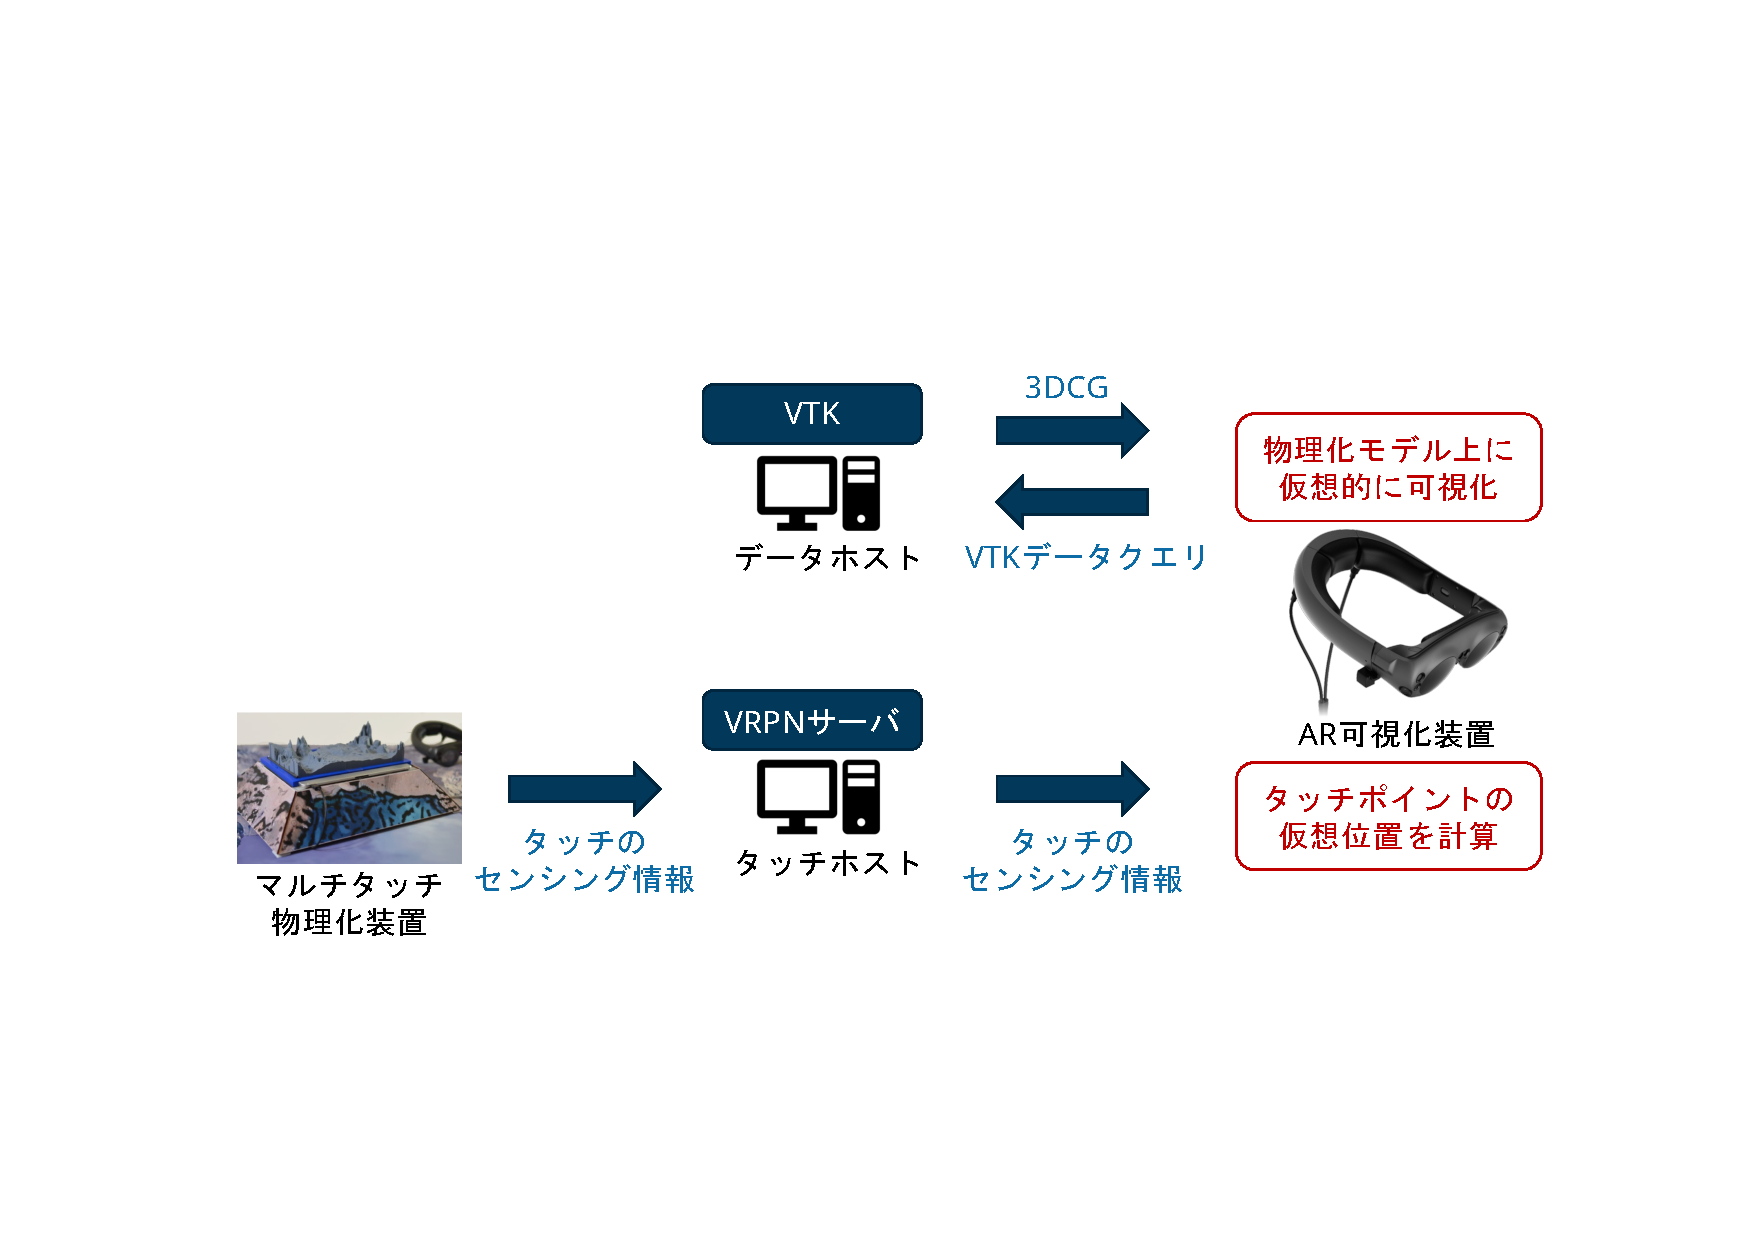
\includegraphics[width=\linewidth]{img/architecture.pdf}
    \caption{提案手法の概要図}
    \label{fig:abstract}
    \end{centering}
\end{figure}

%---------------------------------------------------------------------
\subsection{AR可視化装置}
\label{AR}
ユーザの視線に対するデータの物理化モデルの位置と回転を常に統合するために,パッシブ・インサイド方式によるオブジェクトのトラッキングを行う.
パッシブ・インサイドアウト方式では,物理化モデルとターゲットの平面画像を同時にカメラの視界に配置することでトラッキングが可能であり,持ち運びと検知範囲の点でパッシブ・アウトサイドイン方式よりも優れている.\par
この方式では一度ARマーカを読み込んだ後,AR可視化装置の位置と向いている角度からAR表示の位置を調整する6DoFトラッキングに切り替えるが,定期的にARマーカを再度読み込ませないとトラッキングの精度が低くなる.
そのため,ARマーカをどの角度から見ても読み込める位置に置く必要がある.
一度に読み込むARマーカの枚数と遅延のトレードオフについて調べると,遅延は枚数が少ないほど短く,精度は1枚でも十分であったため,一度に読み込むARマーカの数は少ない方が良いことが分かった.
しかし,全ての角度から1枚のARマーカを読み込むことは不可能であるため,傾斜角が40°のピラミッド型の各側面の中心にARマーカを貼ったステージを使用する\cite{40°}.

%---------------------------------------------------------------------
\subsection{マルチタッチ物理化装置}
\label{マルチタッチ物理化装置}
3Dプリンタで出力した物理化モデルに対するマルチタッチを認識するために,半径0.75cmの六角柱に分割した物理化モデルを高解像度の感圧センサ上に配置する.
半径0.75cmは人間の指先の半径に近い大きさでありながら,物理化モデルの列の数が管理しやすい大きさである.
また,六角形は正方形や長方形と比較して視覚的に硬直した印象を与えづらいため採用した.\par
特定の六角柱が押し下げられた際に,六角柱の端が互いに接触することによって,複数のタッチポイントが登録されてしまうゴーストタッチが発生する場合がある.
提案システムでは,2本の指が同じ六角柱に触れることはないと仮定し,直径が1.5cmよりも小さいタッチポイントが登録された場合,その複数ポイント内で最も大きな力で押し下げられた点のみを残してその他は排除することでゴーストタッチを防ぐ.
また,物理化モデルの重みなどの物理的要因でのゴーストタッチを防ぐため,他のタッチポイントよりも力が5倍以上小さく,力が0.98N未満のものは無視する.

%---------------------------------------------------------------------
%\subsection{動作手順}
%\begin{enumerate}
%\item マルチタッチ物理化装置の近くでARデバイスを装着
%\item ユーザがモデルに触れると,Sensel Morphが感知してVRPNサーバからAR可視化装置にデータを中継
%\item AR可視化装置で各タッチポイントの適切な仮想位置を計算
%\item アフィン変換でタッチポイントをデータに変え,VTKデータクエリを合成しデータホストに送信
%\item データホスト上でVTKを用いて計算し,データの幾何学的表現をAR可視化装置に送信してディスプレイに表示
%\end{enumerate}

%---------------------------------------------------------------------
%\subsection{流線生成の対話性}
%モデル表面の流体の動きをシミュレーションするとき,モデル表面にシード点という点を置き,その点に沿った流線を確認するという方法で行う.
%この時,自分がどこをタッチしているかという情報は重要なため,タッチポイントを分かりやすくするために水平方向に垂直な白い線分を表示する.

%---------------------------------------------------------------------
%\subsection{切断面との対話性}
%切断面を確認することは3Dデータの探索において重要である.切断面は二つのタッチポイントで定義され,二つの点を結ぶ直線の垂直方向の平面で定義される.ユーザが手を話すまで調整可能で,手を離すと座標をデータサーバに送信し,VTKコンポーネントを使用して,切断面をAR可視化装置で表示する.

%---------------------------------------------------------------------
\section{評価}
\subsection{タッチ精度}
提案システムのデータの物理化によるタッチ精度の低下の影響を評価するため,タッチターゲットへのポインティングの8名の被験者実験を行なった.
被験者は,30回のタッチの訓練課題の後,直接感圧センサにタッチするnophysの30回と感圧センサ上の物理化モデル越しにタッチするphysの30回を,それぞれを1セットずつ行なった.
学習効果を最小にするため,nophysとphysの順は4名ずつ入れ替えた.
タッチターゲットは直径5mmで,24cm x 13.85cmの感圧センサにランダムな一様分布で上から投影される.
physでは,ランダムに分布する50個のガウス峰により,最大高さ8mmの凸凹面を持つ地形データを物理化し,その上にタッチターゲットを投影する.
タッチターゲットは一つずつ投影され,あるポイントへのタッチが完了すると次のポイントを表示する.
各タッチターゲットの正解座標とタッチ座標のユークリッド距離を測定し,条件間での平均のタッチ精度を測定した.\par
実験の結果を\figref{fig:touch}に示す.
phys($\mu$ = 3.22mm, $\sigma$ = 2.1mm)と比較して,nophys($\mu$ = 3.09mm, $\sigma$ = 1.64mm)ではより正確にタッチすることができた.
しかし,ウィルコクソンの符号順位検定の結果,データの物理化はタッチ精度に有意な影響を及ぼさず(p = 0.753),「条件間の平均タッチ精度に差がない」という帰無仮説は棄却できなかった.

\begin{figure}[t]
	\begin{centering}
    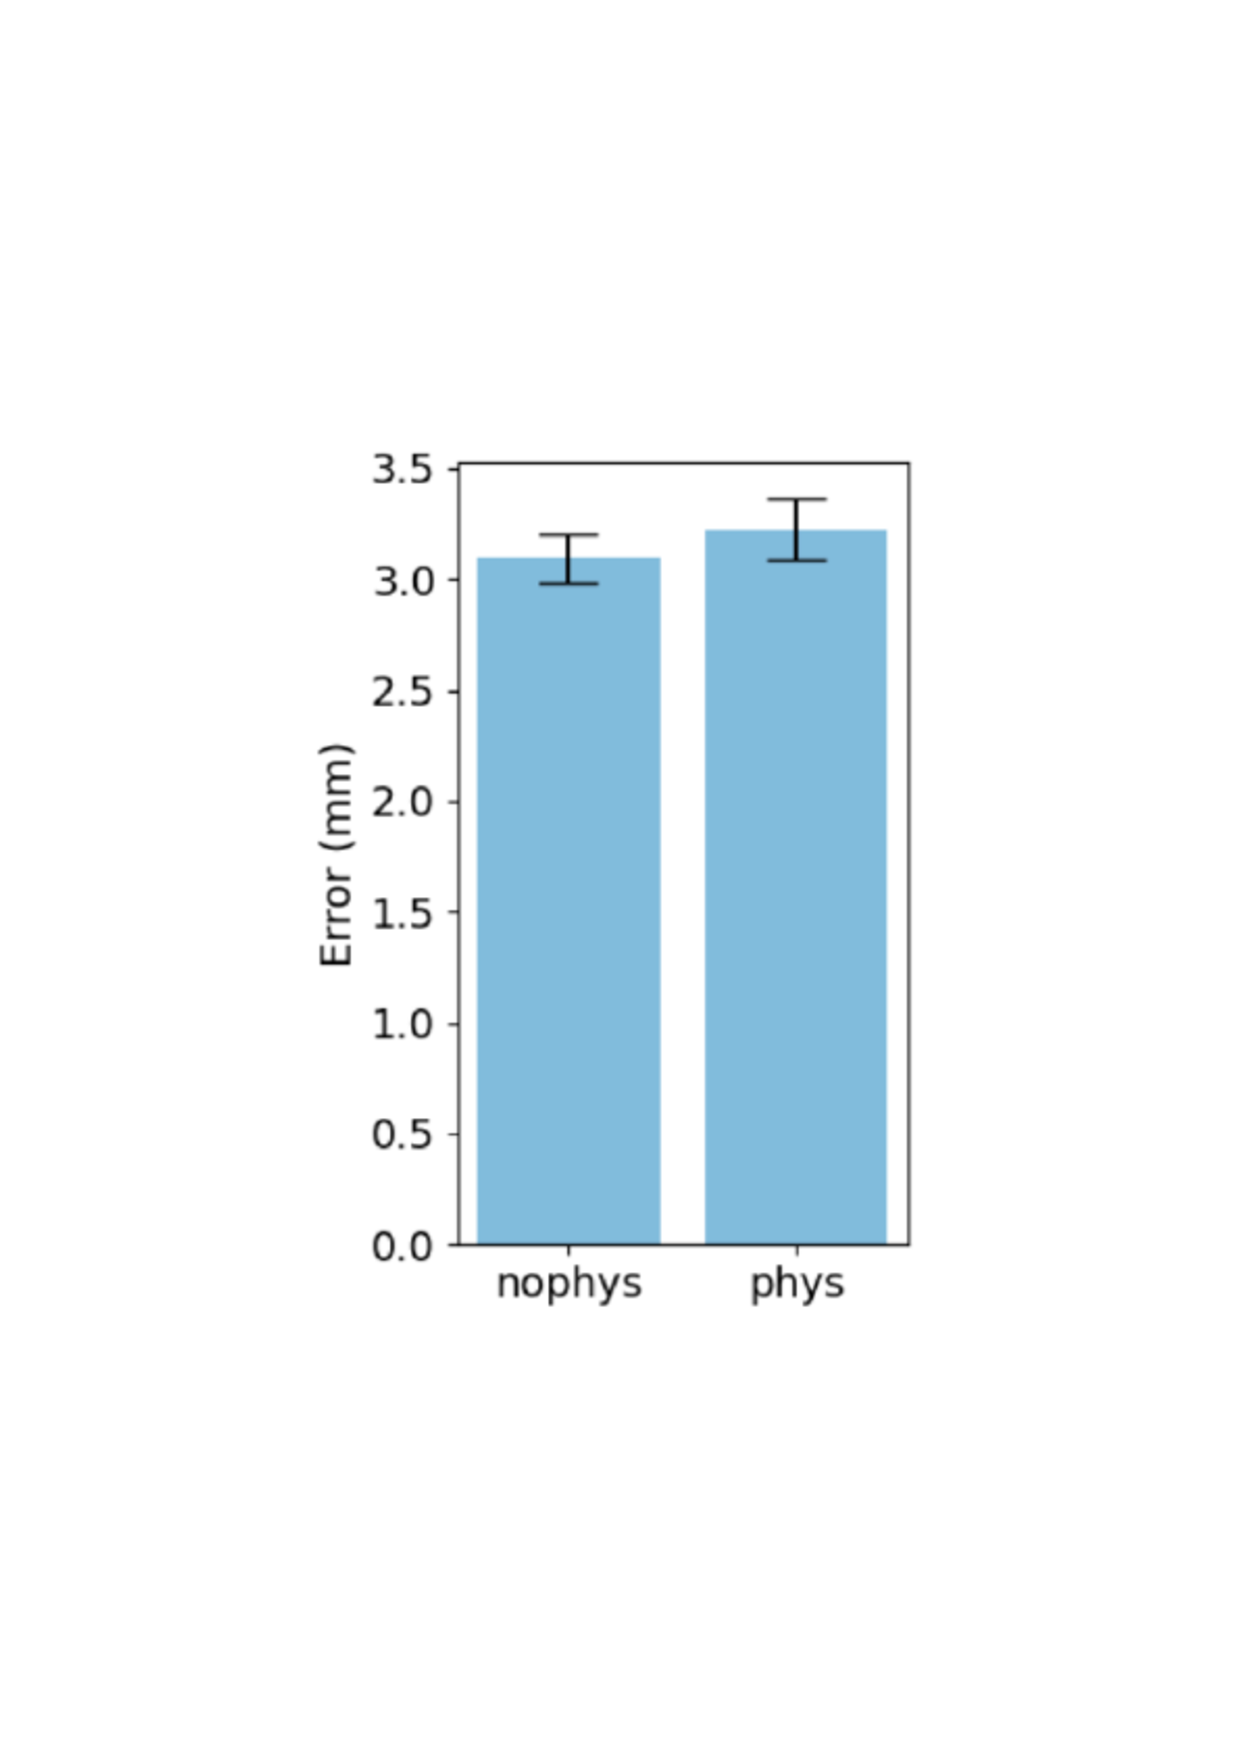
\includegraphics[width=0.35\linewidth]{img/touch.pdf}
    \caption{タッチ精度の実験結果}
    \label{fig:touch}
    \end{centering}
\end{figure}

\subsection{南極気候科学への応用}
データの物理化の実際の科学における可能性を評価するため,南極大陸にあるフィルヒナー・ロンネ棚氷の融解速度を研究する気候科学者にデータの物理化を用いた研究を行ってもらい,思考発話法によるインタビューを行なった.
データの物理化の対象は,気候科学者との相談に基づき,945km x 545kmの小区画を選択した.
元の座標空間からステレオグラフ投影,60倍の垂直方向の拡張,感圧センサのサイズへの切り抜きと拡大縮小等の変換を行い,\ref{マルチタッチ物理化装置}節で説明するように六角柱に分割した.
表面データの六角柱は高さ0.15mmで3Dプリントし,247個の表面データの合計プリント時間は約2日だった.
物理的な可視化と仮想上の可視化の位置合わせを行うトラッキング画像にはNASAの衛星画像を使用しており,南極大陸の鳥瞰図に対するデータと物理化モデルの位置と向きの情報が追加されている.\par
気候科学者へのインタビューは,構築したシステムを使用してもらい,システムの能力を示すための一連の導入タスクを行う中で,思考発話法により行なった.
さらに,システム全体に対する建設的な批判とシステムの使用状況に関するフィードバックの両方を促す質問を,気候科学者の探索プロセス全体にわたって行なった.
インタビューの結果,データが物理的に重なるため直感的理解に役立ち,このシステムを中心としたチームメンバの相互的なコミュニケーションに役立つ可能性があると指摘された.
また,物理化モデルは細かな探索の対象となる主要なデータそのものではなく,3次元の空間マーカとして,より関心のある周辺の対象への方位確認等に用いられていた.

%---------------------------------------------------------------------
\section{まとめと今後の課題}
現在のデータの物理化はデータを伝達する能力は優れているが,ユーザがデータに動的に検索をかける対話的な探索を行うことができない.
本論文では,没入型ARと3Dプリントデータの物理化によるタッチセンシングの作成を組み合わせることで,対話的な探索を支援する物理と仮想のハイブリッド可視化を提案した.
タッチ精度の評価と南極気候科学への応用の実験により,提案システムの有効性を示した.

%---------------------------------------------------------------------
% Bibliography(参考文献)
%---------------------------------------------------------------------
% thebibliography を利用する場合は以下を使用
\footnotesize{
  \begin{thebibliography}{99}
    \bibitem{hybrid} Yvonne Jansen, Pierre Dragicevic and Jean-Daniel Fekete, Evaluating the efficiency of physical visualizations, \textit{Proceedings of the SIGCHI Conference on Human Factors in Computing Systems}, pp.2593-2602, 2013.
    \bibitem{40°} Daniel F Abawi, Joachim Bienwald and Ralf Dorner, Accuracy in optical tracking with fiducial markers: anaccuracy function for ARToolKit, \textit{Third IEEE and ACM International symposium on mixed and augmented reality}, pp.260-261, 2004.
  \end{thebibliography}
}

% BibTex を利用する場合は以下を使用(初めての人には難しいかも)
% \bibliographystyle{junsrt}
% \bibliography{myref}

%---------------------------------------------------------------------
\end{document}
%---------------------------------------------------------------------
